% Results section; every number is a macro generated from results/*.json by python -m telepathy.report.
\begin{table*}[t]
\centering
\caption{Main results. Within-day: velocity $R^2$ on the held-out last 30\,\% of each
calibration day, mean $\pm$ sd over 3 seeds (GRU, SLD) or over the 5 calibration days (linear
decoders). Cross-day: mean $\pm$ sd over the 19 held-out days (days 20--\maxDay), with no labels;
``fixed'' keeps the last calibration day's normalisation; ``adapted'' is re-centring (Wiener,
Kalman, GRU, SLD), FA/Procrustes alignment, or SLD's unsupervised alignment. Bitrate: simulated
WebGrid, click selection, mean $\pm$ sd over 4 sessions of 60\,s after per-decoder tuning.
\textbf{All bitrates come from the simulator, not from a person or animal.}}
\label{tab:main}
\small
\begin{tabular}{lcccc}
\toprule
Decoder & Within-day $R^2$ & \multicolumn{2}{c}{Cross-day $R^2$ (19 days, no labels)} & Sim.\ bits/s \\
 & & fixed & adapted & (10$\times$10) \\
\midrule
Wiener filter (per day) & 0.529 $\pm$ 0.015 & -- & -- & -- \\
Kalman filter (per day) & 0.294 $\pm$ 0.061 & -- & -- & -- \\
Wiener filter (5 days) & 0.528 $\pm$ 0.030 & -0.130 $\pm$ 0.575 & 0.353 $\pm$ 0.207 & 1.27 $\pm$ 0.37 \\
Kalman filter (5 days) & 0.193 $\pm$ 0.021 & -1.894 $\pm$ 2.417 & 0.064 $\pm$ 0.225 & 0.00 $\pm$ 0.00 \\
FA stabiliser~\cite{degenhart2020stabilization} & 0.412 $\pm$ 0.022 & 0.086 $\pm$ 0.338 & 0.235 $\pm$ 0.212 & -- \\
GRU & 0.788 $\pm$ 0.006 & 0.299 $\pm$ 0.154 & 0.589 $\pm$ 0.223 & 1.66 $\pm$ 0.11 \\
SLD (proposed), re-centred & 0.791 $\pm$ 0.007 & 0.388 $\pm$ 0.183 & 0.636 $\pm$ 0.244 & 1.35 $\pm$ 0.18 \\
SLD (proposed), aligned & -- & -- & 0.603 $\pm$ 0.349 & -- \\
Oracle (perfect decoder) & -- & -- & -- & 4.70 $\pm$ 0.17 \\
\bottomrule
\end{tabular}

\end{table*}

\subsection{Within-day decoding}
Table~\ref{tab:main} and Fig.~\ref{fig:within} show that both recurrent decoders are far ahead
of the linear ones: SLD reaches $R^2=\sldWithin$ and the GRU \gruWithin{}, against \wienerWithin{}
for a Wiener filter trained on the same five days. The steady-state velocity Kalman filter is
weak at 20\,ms bins: its smoothing either lags the movement or passes noise, and the
validation-tuned compromise stays below the Wiener filter (Section~\ref{sec:discussion}).
Within one day, SLD and the GRU are statistically indistinguishable (seed sd $\approx$0.007);
the proposed parts of SLD are not meant to win here.

\begin{figure}[t]
\centering
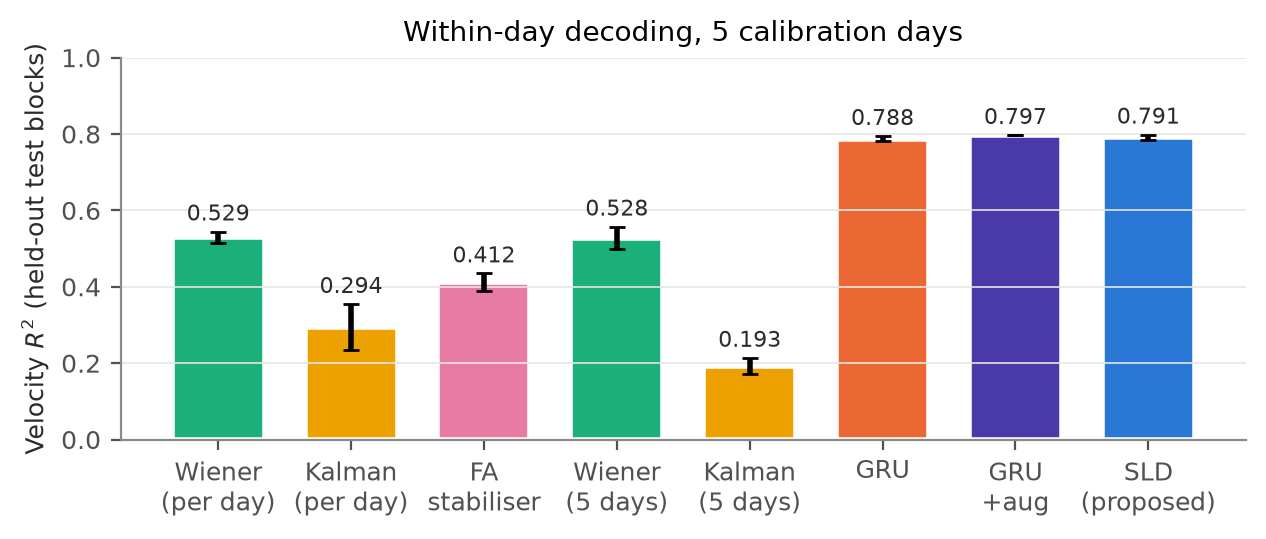
\includegraphics[width=\columnwidth]{figures/fig_within_day.png}
\caption{Within-day velocity $R^2$ on the calibration days' test blocks (error bars: sd over
calibration days or seeds).}
\label{fig:within}
\end{figure}

\subsection{Across days without labels}
\begin{figure*}[t]
\centering
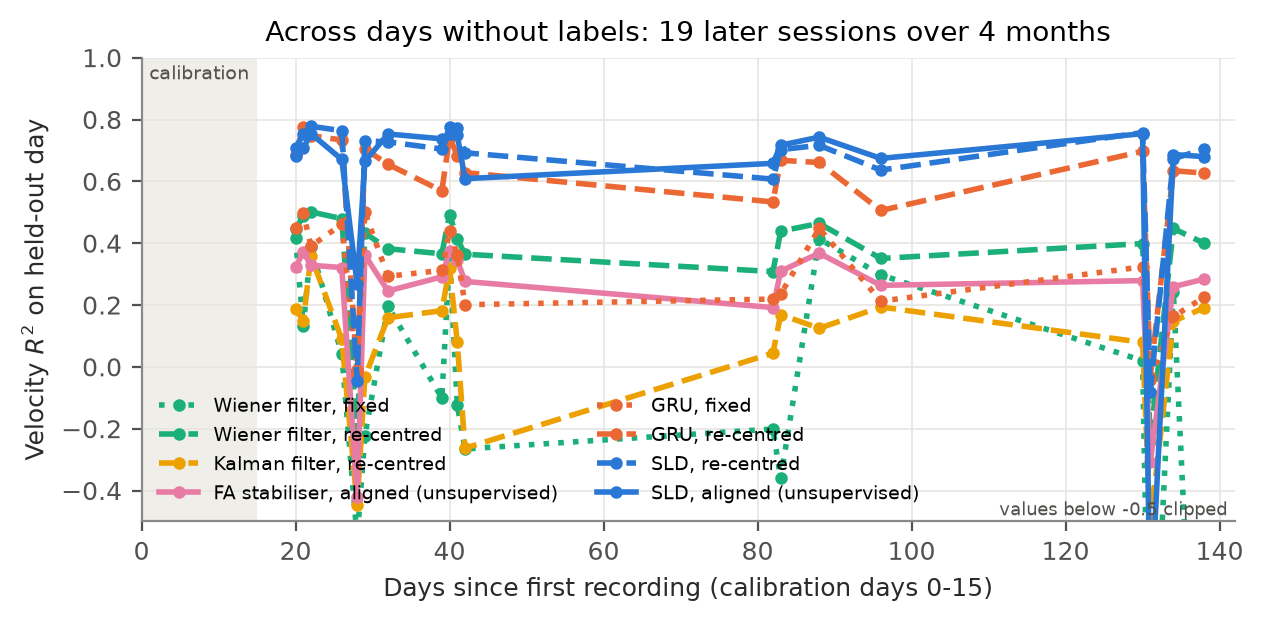
\includegraphics[width=0.78\textwidth]{figures/fig_cross_day.png}
\caption{Velocity $R^2$ on each held-out day, no labels. Dotted: fixed decoder; dashed:
re-centred; solid: unsupervised alignment. Days \flaggedDays{} are electrode re-mapping events
(Sec.~\ref{sec:remap}); every re-centred decoder collapses there.}
\label{fig:cross}
\end{figure*}

Fig.~\ref{fig:cross} tracks every decoder over four months. A fixed Wiener filter is unusable
(mean $R^2=\allWienerFixed$; individual days fall below $-1$), and even the recurrent decoders
lose roughly half their accuracy when left fixed (GRU \allGruFixed, SLD \allSldFixed). Re-centring
each channel with the new day's unlabelled statistics recovers most of the loss. On the
\nKeep{} days without an electrode re-mapping, re-centred SLD averages
$R^2=\keepSldRc$ and the re-centred GRU \keepGruRc, close to their within-day accuracy, while the
Wiener filter reaches \keepWienerRc{} and the FA stabiliser \keepFaAligned.

\paragraph{What makes a decoder hold up?} The ablation (Table~\ref{tab:ablation}) separates
the ingredients. Training with Sussillo-style input perturbations is worth about
+0.05 $R^2$ across days for the GRU (\keepGruRc{} $\to$ \keepGruAugRc), and SLD inherits it;
removing augmentation from SLD costs less across days (\keepSldNoAugRc{} vs \keepSldRc), possibly
because the masked-spike loss also exposes it to missing channels. The per-day adapters and the
masked-spike loss make no measurable difference to re-centred accuracy
(\keepSldNoAdaptersRc{} without adapters, \keepSldNoSslRc{} without the loss), and the banded
transformer backbone is slightly worse than the GRU (\keepSldTransformerRc).

\paragraph{Does unsupervised alignment help?} Mostly not, on natural drift. Averaged over
the \nKeep{} regular days, aligned SLD (\keepSldAligned) is no better than re-centred SLD (\keepSldRc).
The effect depends on elapsed time: within six weeks of calibration alignment costs
\alignGainEarly{} $R^2$ on average, while 82--138 days out it gains \alignGainLate. Starting from
the re-centred decoder and penalising departures from the identity limits the damage, but the
objective (spike likelihood plus latent-moment matching) is not tied to velocity, so when the
re-centred decoder is already good it can only move away from it.

\begin{table*}[t]
\centering
\caption{Ablations (velocity $R^2$). Within-day: test blocks of the calibration days. Cross-day
means exclude the two re-mapping days; aligned variants of single-seed ablations were run on a
7-day subset (days \ablSubsetDays), so the last two columns compare all models on that subset.}
\label{tab:ablation}
\small
\begin{tabular}{lccccc}
\toprule
Model & Within-day & \multicolumn{2}{c}{Cross-day, 17 days} & \multicolumn{2}{c}{Cross-day, 7-day subset} \\
 & & fixed & re-centred & aligned & re-centred \\
\midrule
SLD (full) & 0.791 $\pm$ 0.007 & 0.433 & 0.718 & 0.715 & 0.734 \\
w/o input augmentation & 0.805 & 0.300 & 0.701 & 0.727 & 0.716 \\
w/o masked-spike loss & 0.784 & 0.447 & 0.711 & 0.702 & 0.727 \\
w/o day adapters & 0.796 & 0.434 & 0.725 & -- & 0.736 \\
transformer backbone & 0.764 & 0.456 & 0.698 & 0.671 & 0.713 \\
GRU baseline & 0.788 $\pm$ 0.006 & 0.337 & 0.662 & -- & 0.679 \\
GRU + augmentation & 0.797 & 0.444 & 0.712 & -- & 0.726 \\
\bottomrule
\end{tabular}

\end{table*}

\subsection{Electrode re-mapping events}
\label{sec:remap}
Two held-out sessions (days \flaggedDays) break every re-centred decoder ($R^2\approx0$). A
decoder trained on that day alone still reaches $R^2>0.5$, so the neurons still encode
velocity; what changed is which electrode records what. A label-free check confirms it: the
correlation between each channel's mean firing rate on the new day and on the last calibration
day is \flagCorr{} on these two days and between \otherCorrMin{} and \otherCorrMax{} on all other
held-out days. This is the situation latent alignment is designed for. On day \flagADay, SLD
alignment recovers $R^2$ = \flagAAligned{} (three seeds) from \flagARc{} re-centred; on day
\flagBDay{} it recovers one seed (\flagBAligned) and makes the others worse. Alignment can find
the re-mapping but is not reliable; in a product it should be gated by the detector above and
verified before it is trusted.

\subsection{Electrode failure and re-wiring}
\begin{figure*}[t]
\centering
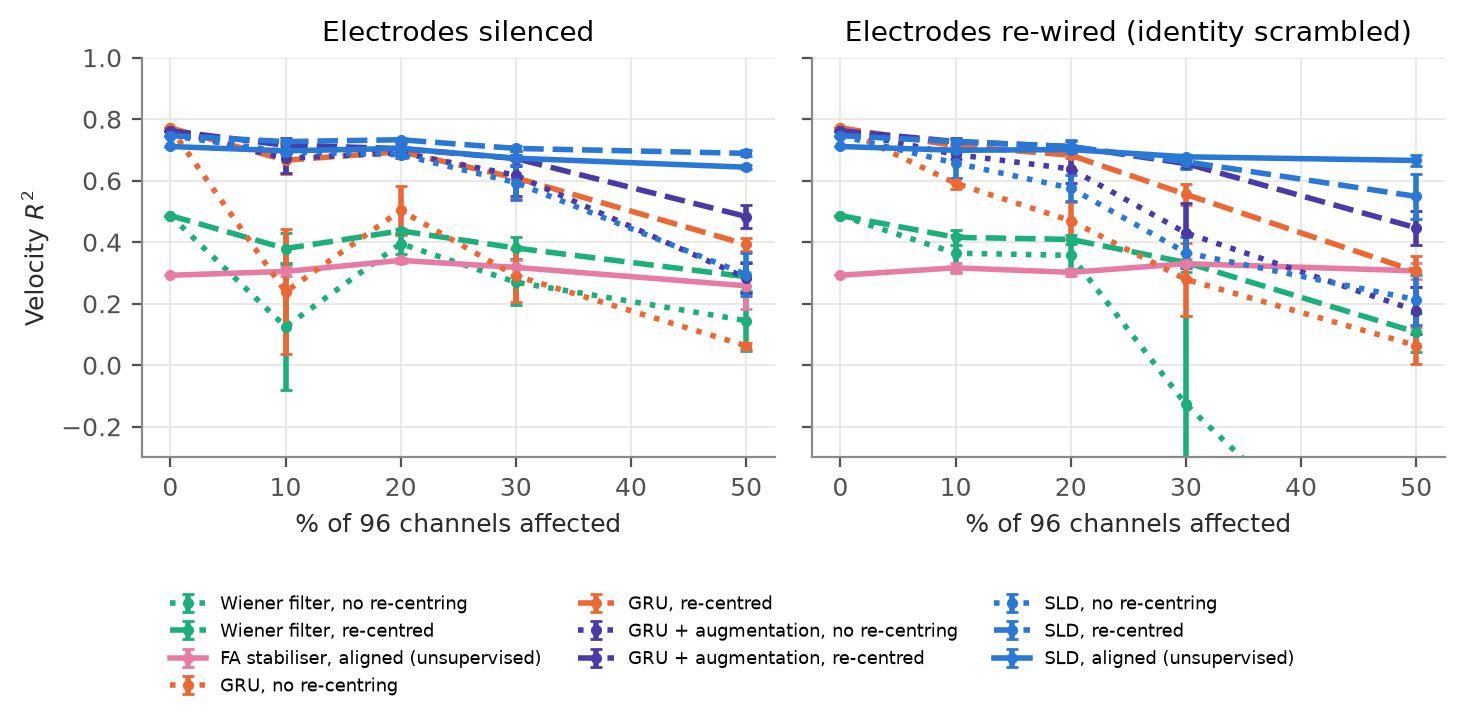
\includegraphics[width=0.85\textwidth]{figures/fig_stress.png}
\caption{Stress tests on the last calibration day: a growing fraction of electrodes silenced
(left) or swapped with each other (right); mean $\pm$ sd over 3 random draws.}
\label{fig:stress}
\end{figure*}
Fig.~\ref{fig:stress} silences or scrambles a growing fraction of the 96 channels. Silencing is
where augmentation matters most. With half the electrodes dead, the plain GRU falls to
$R^2=\stDropGruNaiveFifty{}$ (\stDropGruRcFifty{} after re-centring), the augmented GRU to
\stDropGruAugRcFifty, while SLD keeps \stDropSldRcFifty. Already at 10\,\% silenced the plain
GRU without re-centring drops to \stDropGruNaiveTen. For re-wired electrodes, re-centring again
does most of the work; unsupervised alignment adds a little at 30\,\% re-wired
(\stShiftSldAlignedThirty{} vs \stShiftSldRcThirty) and nothing at small fractions.

\subsection{Few-shot recalibration}
\begin{figure}[t]
\centering
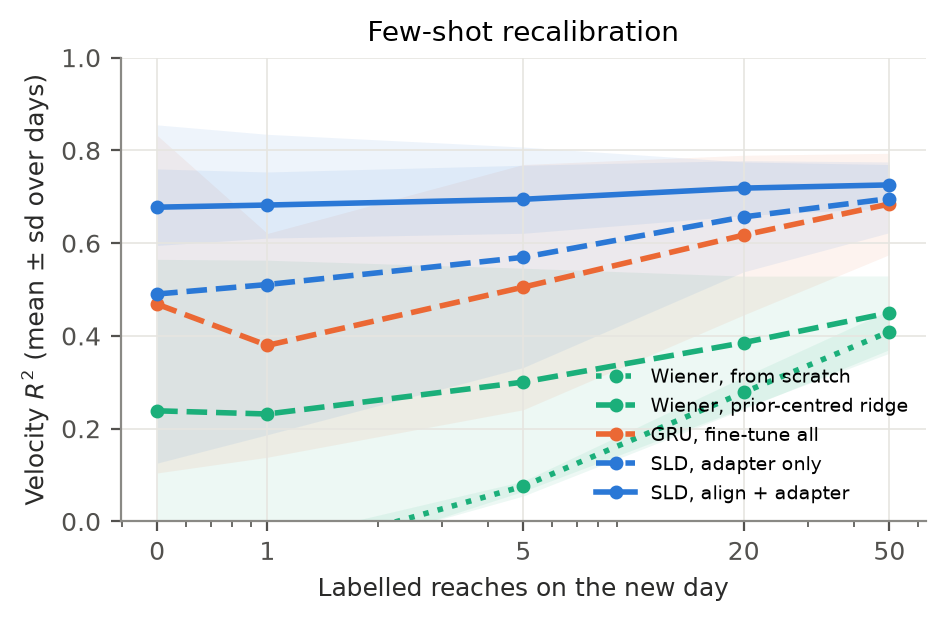
\includegraphics[width=\columnwidth]{figures/fig_fewshot.png}
\caption{Few-shot recalibration on \fsDays{} held-out days (days 20, 28 and 40; day 28 is a
re-mapping day; one seed). $N=0$ is the label-free starting point of each method.}
\label{fig:fewshot}
\end{figure}
\begin{table*}[t]
\centering
\caption{Few-shot recalibration ($R^2$, mean $\pm$ sd over \fsDays{} held-out days: 20, 28 and 40; one seed; CPU budget).}
\label{tab:fewshot}
\small
\begin{tabular}{lccccc}
\toprule
Method & $N=0$ & $N=1$ & $N=5$ & $N=20$ & $N=50$ \\
\midrule
Wiener, from scratch & -- & -0.08 $\pm$ 0.04 & 0.08 $\pm$ 0.01 & 0.28 $\pm$ 0.03 & 0.41 $\pm$ 0.05 \\
Wiener, prior-centred ridge & 0.24 $\pm$ 0.33 & 0.23 $\pm$ 0.33 & 0.30 $\pm$ 0.25 & 0.39 $\pm$ 0.14 & 0.45 $\pm$ 0.08 \\
GRU, fine-tune all & 0.47 $\pm$ 0.36 & 0.38 $\pm$ 0.24 & 0.51 $\pm$ 0.26 & 0.62 $\pm$ 0.17 & 0.68 $\pm$ 0.11 \\
SLD, adapter only & 0.49 $\pm$ 0.36 & 0.51 $\pm$ 0.32 & 0.57 $\pm$ 0.24 & 0.66 $\pm$ 0.12 & 0.70 $\pm$ 0.07 \\
SLD, align + adapter & 0.68 $\pm$ 0.08 & 0.68 $\pm$ 0.07 & 0.69 $\pm$ 0.07 & 0.72 $\pm$ 0.06 & 0.73 $\pm$ 0.05 \\
\bottomrule
\end{tabular}

\end{table*}
With labels, the question becomes how few reaches are needed (Fig.~\ref{fig:fewshot},
Table~\ref{tab:fewshot}). A Wiener filter trained from scratch is useless with 1--5 reaches and
still poor at 50. Shrinking toward the calibrated weights is safe but slow. Fine-tuning every
GRU weight on one reach damages the decoder ($R^2$ \fsGruFinetuneNOne{} vs \fsGruFinetuneNZero{}
at $N=0$). Fitting only SLD's day adapter is stable at every $N$ (\fsSldFewshotNOne{} at $N=1$,
\fsSldFewshotNFifty{} at $N=50$), and starting it from the unsupervised alignment gives the best
curve (\fsSldAlignFewshotNTwenty{} at $N=20$), largely because it rescues the re-mapping day in the sample.

\subsection{Closed loop: simulated WebGrid}
\begin{figure}[t]
\centering
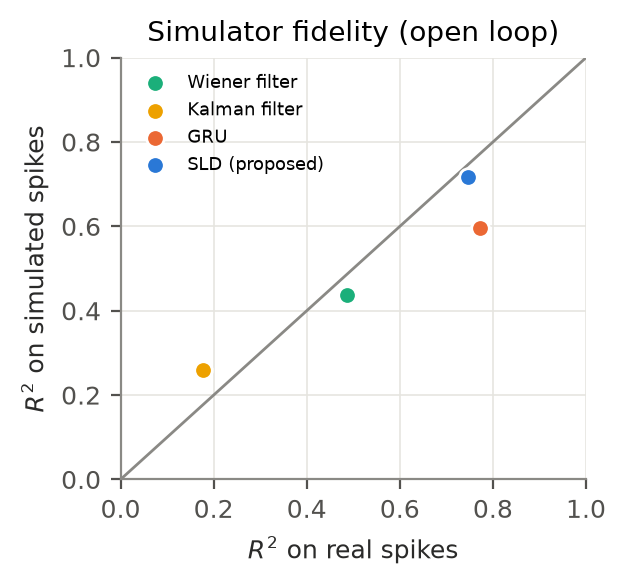
\includegraphics[width=0.75\columnwidth]{figures/fig_sim_fidelity.png}
\caption{Simulator fidelity: each decoder's $R^2$ on real test spikes vs on simulated spikes
generated from the same velocities.}
\label{fig:fidelity}
\end{figure}

\paragraph{Fidelity.} With the noise scale calibrated on the Wiener filter, the simulated spikes
reproduce the linear decoders' accuracy (Wiener \fidWienerReal{} real vs \fidWienerSim{}
simulated) and SLD's (\fidSldReal{} vs \fidSldSim), but the GRU loses more in simulation
(\fidGruReal{} vs \fidGruSim): the encoder does not reproduce every feature the GRU relies on
(Fig.~\ref{fig:fidelity}).

\begin{figure*}[t]
\centering
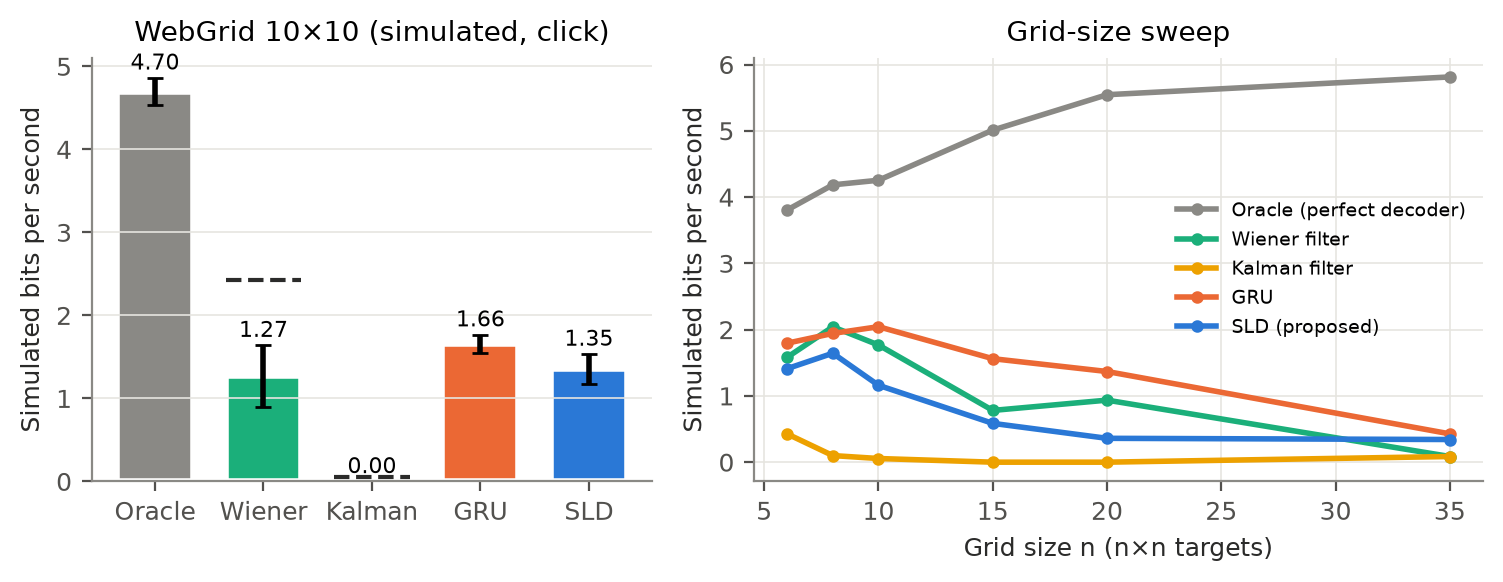
\includegraphics[width=0.85\textwidth]{figures/fig_webgrid_bps.png}
\caption{Simulated WebGrid bitrate. Left: \gridSize$\times$\gridSize{} grid, 4 sessions of
60\,s per decoder; dashed bars mark the linear decoders after ReFIT-style recalibration.
Right: bitrate vs grid size (30\,s sessions).}
\label{fig:bps}
\end{figure*}
\begin{figure*}[t]
\centering
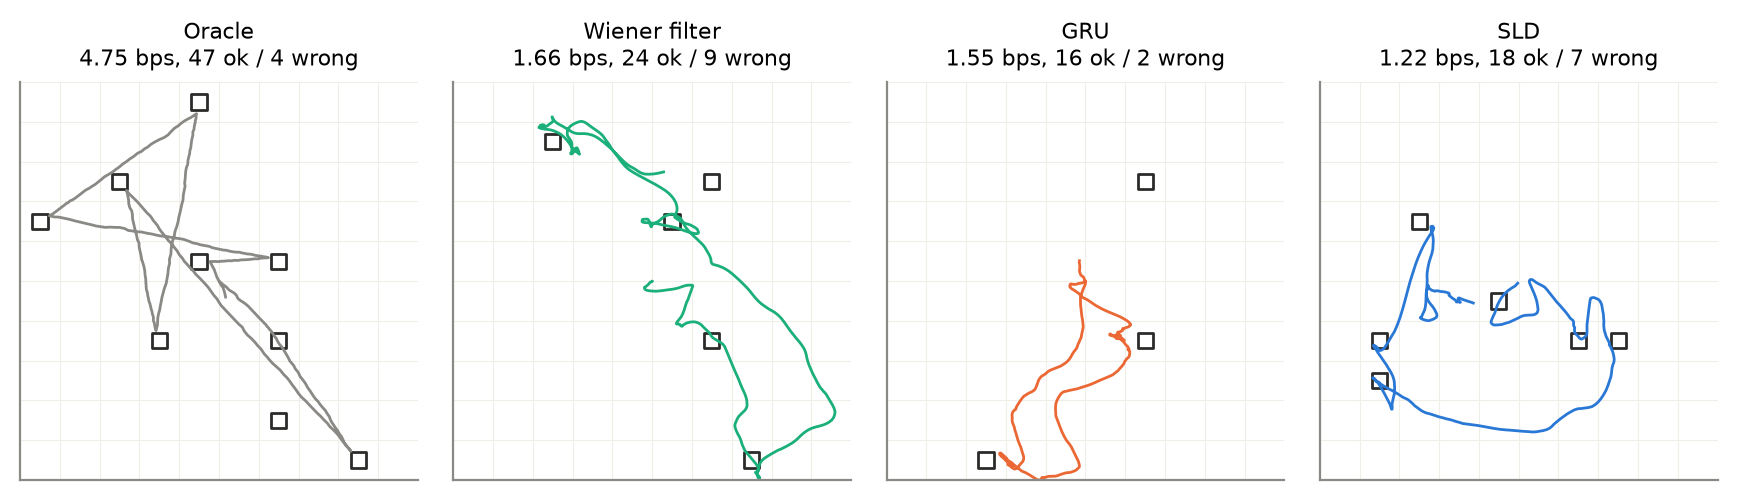
\includegraphics[width=0.85\textwidth]{figures/fig_webgrid_traces.png}
\caption{First 10\,s of one simulated session per decoder (squares: targets).}
\label{fig:traces}
\end{figure*}

\paragraph{Bitrate.} Fig.~\ref{fig:bps} and Table~\ref{tab:cl} give the main closed-loop
result. A perfect decoder at the same latency scores \oracleBps{} bits/s on the
\gridSize$\times$\gridSize{} grid, the ceiling set by the user model and the task. The GRU scores
\gruBps, SLD \sldBps, the Wiener filter \wienerBps{} and the Kalman filter \kalmanBps. Offline
ranking does not carry over cleanly: SLD and the GRU are tied offline and the GRU scores slightly
higher in closed loop, while the much less accurate Wiener filter comes close to SLD once its
output is smoothed. The
spread between the SLD ablations is as large as the differences between decoders
(\simAblSldNoAdapters{} bits/s without adapters, \simAblSldNoAug{} without augmentation,
\simAblSldNoSsl{} without the masked-spike loss, \simAblSldTransformer{} with the transformer;
GRU with augmentation \simAblGruAug), so differences below about 0.5 bits/s should not be read as
real with four 60\,s sessions. What is robust: every neural decoder beats the Kalman filter by a
wide margin, the best decoder reaches only about a third of the perfect-decoder ceiling
(\gruBps{} vs \oracleBps{} bits/s), and precision,
not speed, limits them, because bitrate falls with grid size for every decoder while it rises for
the oracle (\sweepOracleGThirtyFive{} bits/s for the oracle on 35$\times$35, \sweepGruGThirtyFive{}
for the GRU). Dwell selection is much worse than clicking for the decoders (Table~\ref{tab:cl}):
holding the cursor still on one small cell for 0.5\,s is hard for a noisy cursor.

\paragraph{ReFIT in simulation.} Recalibrating the Wiener filter on 120\,s of its own
closed-loop data with intention relabelling lifts it from \wienerBps{} to \wienerRefitBps{}
bits/s, the qualitative effect Gilja et al.\ reported in monkeys~\cite{gilja2012refit}. That the
simulator reproduces a known closed-loop effect that offline metrics cannot show is the best
evidence that it is useful. The same procedure does not rescue the Kalman filter
(\kalmanRefitBps{} bits/s), whose problem here is its offline fit, not intention labels.

\begin{table}[t]
\centering
\caption{Closed-loop details: tuned gain, velocity smoothing and click hold time per decoder;
simulated bits/s with click and with 0.5\,s dwell selection (\gridSize$\times$\gridSize).}
\label{tab:cl}
\scriptsize
\setlength{\tabcolsep}{2.5pt}
\resizebox{\columnwidth}{!}{\begin{tabular}{lccccc}
\toprule
Decoder & gain & smooth & hold (s) & click bits/s & dwell bits/s \\
\midrule
Oracle & 1 & 0 & 0.1 & 4.70 $\pm$ 0.17 & 4.20 $\pm$ 0.21 \\
Wiener & 0.75 & 0.6 & 0.1 & 1.27 $\pm$ 0.37 & 0.55 $\pm$ 0.45 \\
Kalman & 1 & 0 & 0.1 & 0.00 $\pm$ 0.00 & 0.00 $\pm$ 0.00 \\
GRU & 1 & 0 & 0.25 & 1.66 $\pm$ 0.11 & 0.00 $\pm$ 0.00 \\
SLD & 1.5 & 0.6 & 0.1 & 1.35 $\pm$ 0.18 & 0.00 $\pm$ 0.00 \\
Wiener + ReFIT & 1 & 0.6 & 0.1 & 2.43 $\pm$ 0.37 & -- \\
Kalman + ReFIT & 0.75 & 0.6 & 0.1 & 0.06 $\pm$ 0.06 & -- \\
\bottomrule
\end{tabular}
}
\end{table}

\paragraph{Across days in closed loop.}
\begin{figure}[t]
\centering
\IfFileExists{figures/fig_crossday_bps.png}{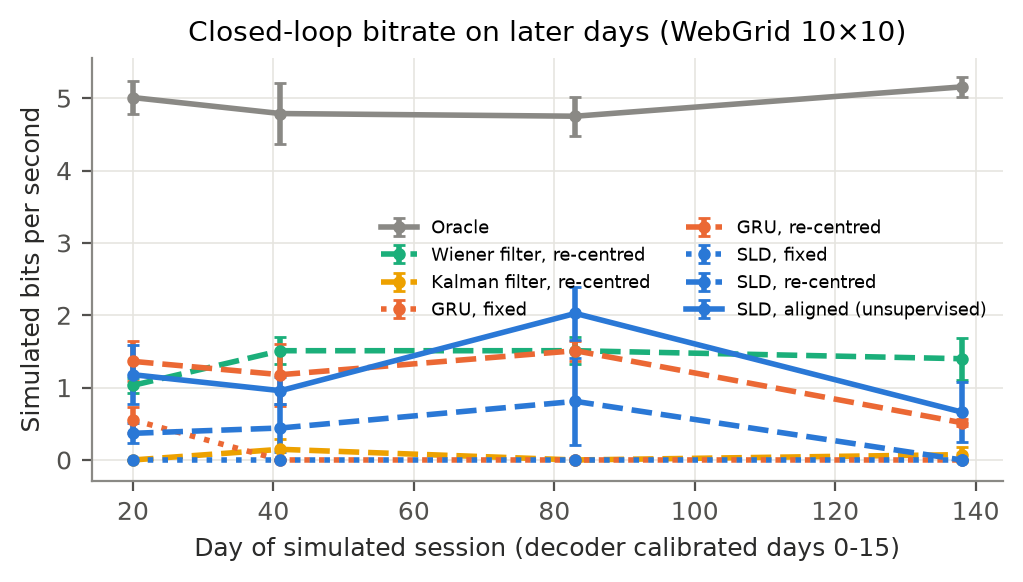
\includegraphics[width=\columnwidth]{figures/fig_crossday_bps.png}}{}
\caption{Simulated bitrate on later days with the decoders' day-0 tuning (3 sessions per point).}
\label{fig:cdbps}
\end{figure}
Fig.~\ref{fig:cdbps} repeats the closed-loop test on four later days, with an encoding model fit
to each day and no re-tuning. Fixed decoders fail outright (mean \cdBpsGruFixed{} bits/s for
the fixed GRU, \cdBpsSldFixed{} for fixed SLD), confirming in closed loop what the offline
numbers show. Re-centring restores the Wiener filter (\cdBpsWienerRc{} bits/s on average) and the
GRU (\cdBpsGruRc). For SLD the closed loop reverses the offline picture: with a fresh identity
adapter and re-centring it scores only \cdBpsSldRc{} bits/s, while the unsupervised-aligned
adapter scores \cdBpsSldAligned{}, although the two differ little in offline $R^2$. The re-centred
Wiener filter is the most consistent decoder across the four days in closed loop; the
neural decoders degrade on the last day (day 138). Four days and three sessions per point are
too few for firm rankings, but the pattern is a second warning against choosing a stabilisation
method on offline $R^2$ alone.

\subsection{Latency}
All decoders are cheap enough for a 20\,ms update on one CPU thread (Table~\ref{tab:latency}):
the GRU and SLD need about 1\,ms per bin, the banded transformer about 5\,ms because it re-reads
its context window at every step.
\begin{table}[t]
\centering
\caption{Streaming inference cost per 20\,ms bin (one CPU thread, shared machine).}
\label{tab:latency}
\scriptsize
\begin{tabular}{lc}
\toprule
Decoder & ms per 20\,ms bin \\
\midrule
Wiener filter & 0.073 \\
Kalman filter & 0.117 \\
FA stabiliser & 2.339 \\
GRU & 0.758 \\
SLD (GRU backbone) & 1.109 \\
SLD (transformer backbone) & 5.541 \\
\bottomrule
\end{tabular}

\end{table}

\begin{figure*}[t]
\centering
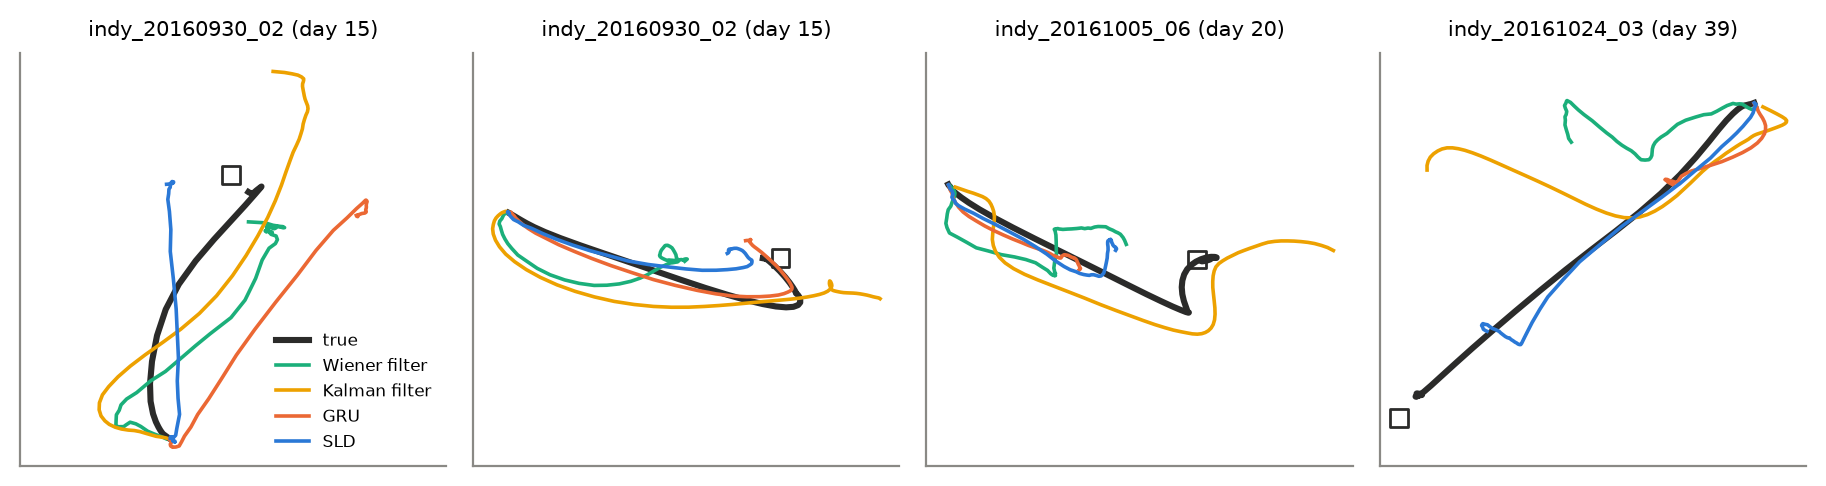
\includegraphics[width=0.9\textwidth]{figures/fig_trajectories.png}
\caption{Held-out reaches: true cursor path (black) and the path obtained by integrating each
decoder's velocity from the true start. Left two: last calibration day. Right two: later days,
re-centred (Wiener, Kalman, GRU) or aligned (SLD), no labels.}
\label{fig:traj}
\end{figure*}
